\chapter{Introduction}
\label{sec:intro}

\cleanchapterquote{Finance is the art of passing currency from hand to hand until it finally disappears.}{Robert W. Sarnoff}{(1918-1997)}

This thesis presents different numerical methods for pricing FX-TARN under L\'evy processes. In general, options with path dependents payoff, such as this product, are evaluated by Monte Carlo simulations. We will describe two other methods based on Finite Difference (FD) and Fast Fourier Transform (FFT). The initial chapter starts, in Section \ref{sec:intro:motivation}, with an historic of existing works that allowed this project to born. Then, in Section \ref{sec:intro:description}, the FX-TARN product is presented. In section \ref{sec:intro:term_sheet}, an example of term sheet illustrates this exotic product. Finally, the chapter concludes with an overview of the thesis in section \ref{sec:intro:overview}.

\section{Motivation}
\label{sec:intro:motivation}
This project was born during my internship in market risk management at Pictet, a swiss private bank. In fact, I had to reprice FX-TARN to evaluate the risk on this product. The first approach was to price it with Monte Carlo simulations. However, the computational cost was very expensive. Several numbers of research brought me to the paper of \citeauthor{LS15} \citeyearpar{LS15}, in which they develop a Finite Difference (FD) method for Black-Scholes model. 

It is well known that the assumptions under Black-Scholes model are too restrictive with respect to the market. Indeed, the log-normality of the returns and the path continuity are contradicted by the analysis of the financial data. We can clearly identify jumps in financial time series. In addition, the implied volatility presents in general a negative skew which means that the returns distribution is more leptokurtic (fat tails) than the normal one. This can be due effectively to the jumps in the market prices, accentuated during the economic crises.

To go beyond the Black-Scholes model and avoid inconsistencies with the markets, we can model stock price with exponential L\'evy processes. There are two different classes of L\'evy models used in this thesis, the jump-diffusion (finite activity) models which are extension of Black-Scholes model including jumps, and pure jump (infinite activity) models which model the asset price by infinitely many small jumps. The advantage of these models is that they capture
the volatility smile structure. 

The first part of the study was thus to enlarge the Finite Difference (FD) method proposed by \citeauthor{LS15} to the L\'evy processes with jumps. This generalization involves the L\'evy measure characterizing the jumps. This leads to large complexities in the implementation of the method and then the computational time grows up with the complexity. Therefore the question was how to boost the pricing engine. The Computational Finance lesson given by the Prof. \citeauthor{Nob15} in collaboration with Prof. Pulido and Kressner from the Swiss Institute of Technology Lausanne (EPFL), gives me the idea to solve the problem with Fast Fourier Transform (FFT). At the end, the solution was found in the Convolution method proposed by \citeauthor{Lor+08} \citeyearpar{Lor+08}, where they apply a FFT based method to the early exercised option like Bermudan or American options. T hen, the combination of the methods of \citeauthor{LS15} and \citeauthor{Lor+08} allows us to develop our own method to price FX-TARN with the FFT approach.

To achieve this project, it was natural to call the Prof. Fabio Nobile, who is a specialist of numerical analysis in partial differential equations (PDE), and the Prof. Julien Hugonnier, who taught me the pricing of financial derivatives. Thank's to them for their useful supervision.

\section{FX-TARN Description}
\label{sec:intro:description}
An FX Target Accrual Redemption Note (FX-TARN) is a financial product that allows an investor to accumulate an amount of cash until a certain \textit{target accrual level} $U$ over a predefined schedule. More precisely, the contract between the bank and the client imposes cash flow on scheduled dates (fixing dates). We can replicate these cash flows with a series of FX call options (resp. FX put options) with strike $K$, that the bank sells to a client, and at the same time a series of FX put options (resp. FX call options) with the same strike $K$, that the bank buys from the client. Sometimes, the client leg that the bank buys is combined with a leverage factor $g$ called \textit{gear factor}. The scheduling is defined by a number of fixing dates $t_1,t_2,\ldots,t_N$ that corresponds to the option expiry dates. Finally, the product knock-out if the total sum of payouts (from the bank's point of view) exceeds the given target $U$. There are three types of knock-out when the target $U$ is breached that we will see in the next section:
\begin{my_list_item}
\item \textbf{No Gain :} the last payment is disallowed when the target $U$ is breached,
\item \textbf{Part Gain :} only a part of the payment is allowed such that only the target is paid,
\item \textbf{Full Gain :} the last payment is allowed when the target $U$ is breached. 
\end{my_list_item}

\subsubsection*{Payoff Definition}
\label{sec:intro:Payoff}
Define the following notations:
\begin{my_list_item}
\item $S(t)$ : FX rate at time $t$,
\item $K$ : strike(s) (could be different for each fixing dates),
\item $t_0$ : today's date,
\item $t_1,t_2,\ldots,t_M$ : fixing dates,
\item $U$ : target accrual level,
\item $A(t)$ : accumulated gains at time $t$,
\item $N_f$ : Accrual amount per fixing date.
\end{my_list_item}

On each fixing date $t_n, n = 1,\ldots,N,$ if the target level $U$ is not breached by the accumulated amount $A(t_m)$, the gain per unit of notional foreign amount from the point of view of the investor is given by
\[\tilde{C}_n = \beta(S(t_n)-K)\times \mathbf{1}_{\{\beta S(t_n)\geq \beta K\}}, \]
and the loss
\[\tilde{C}_n^\ast = -g \times \beta(K-S(t_n))\times \mathbf{1}_{\{\beta S(t_n)\leq \beta K\}}, \]
where $\beta$ is the strategy, i.e. $\beta = 1$ the investor buys call options, $\beta = -1$ the investor buys put options.

Denote $t_{\tilde{N}}$ the first fixing date before maturity on which the target level $U$ is breached by the total accumulated gain (without the loss part), i.e.
\[\tilde{N}=\min\{n: A(t_n)\geq U\},\qquad n = 1,2,\ldots,N.\]
If the target $U$ is not breached, set $\tilde{N} = N$. For $t_n \leq t_{\tilde{N}}$ we can write the actual payment for a gain as
\begin{equation}\label{eq:TARN:gain}
C_n(S(t_n),A(t_{n-1})) = \tilde{C}_n\times \left(\mathbf{1}_{\{A(t_{n-1}))+\tilde{C}<U\}}+W_n\times\mathbf{1}_{\{A(t_{n-1})+\tilde{C}\geq U\}}\right),
\end{equation}
and $C_n=0$ for $t_n>t_{\tilde{N}}$. The loss does not count in the knock-out condition but will also knock-out by the same redemption event. Therefore we have that
\begin{equation}\label{eq:TARN:loss}
C^\ast_n(S(t_n),A(t_{n-1})) = \tilde{C}_n^\ast\times \left(\mathbf{1}_{\{A(t_{n-1})+\tilde{C}<U\}}+W_n\times\mathbf{1}_{\{A(t_{n-1})+\tilde{C}\geq U\}}\right).
\end{equation}
Here, $A(t_{n-1})$ is the accumulated gain immediately after the fixing date $t_{n-1}$ and $W_n$ is the weight corresponding to the type of knock-out when the target is breached. We can set the weights $W_n$ for the different types of knock-out as follow:
\[W_n = \begin{cases}
0, &\text{for No Gain,} \\
\frac{U-A(t_{n-1})}{\beta\times(S(t_n)-K)}, & \text{for Part Gain,}\\
1, &\text{for Full Gain.}
\end{cases}\]

Therefore, the accumulated gains $A(t)$ is a step function such that $A(t) = A(t_{n-1})$, for $t_{n-1}\leq t < t_n$ with
\[A(t_n)= A(t_{n-1}) + C_n(S(t_n),A(t_{n-1})).\]
In Figure \ref{fig:cash-flow}, we can see the plot of the positive cash flow $C(S(t),A(t^-)) = C(S,A)$ that counts in the accumulated amount and produces jumps in the price on a fixing date.
\begin{figure}[!htb]
\centering
	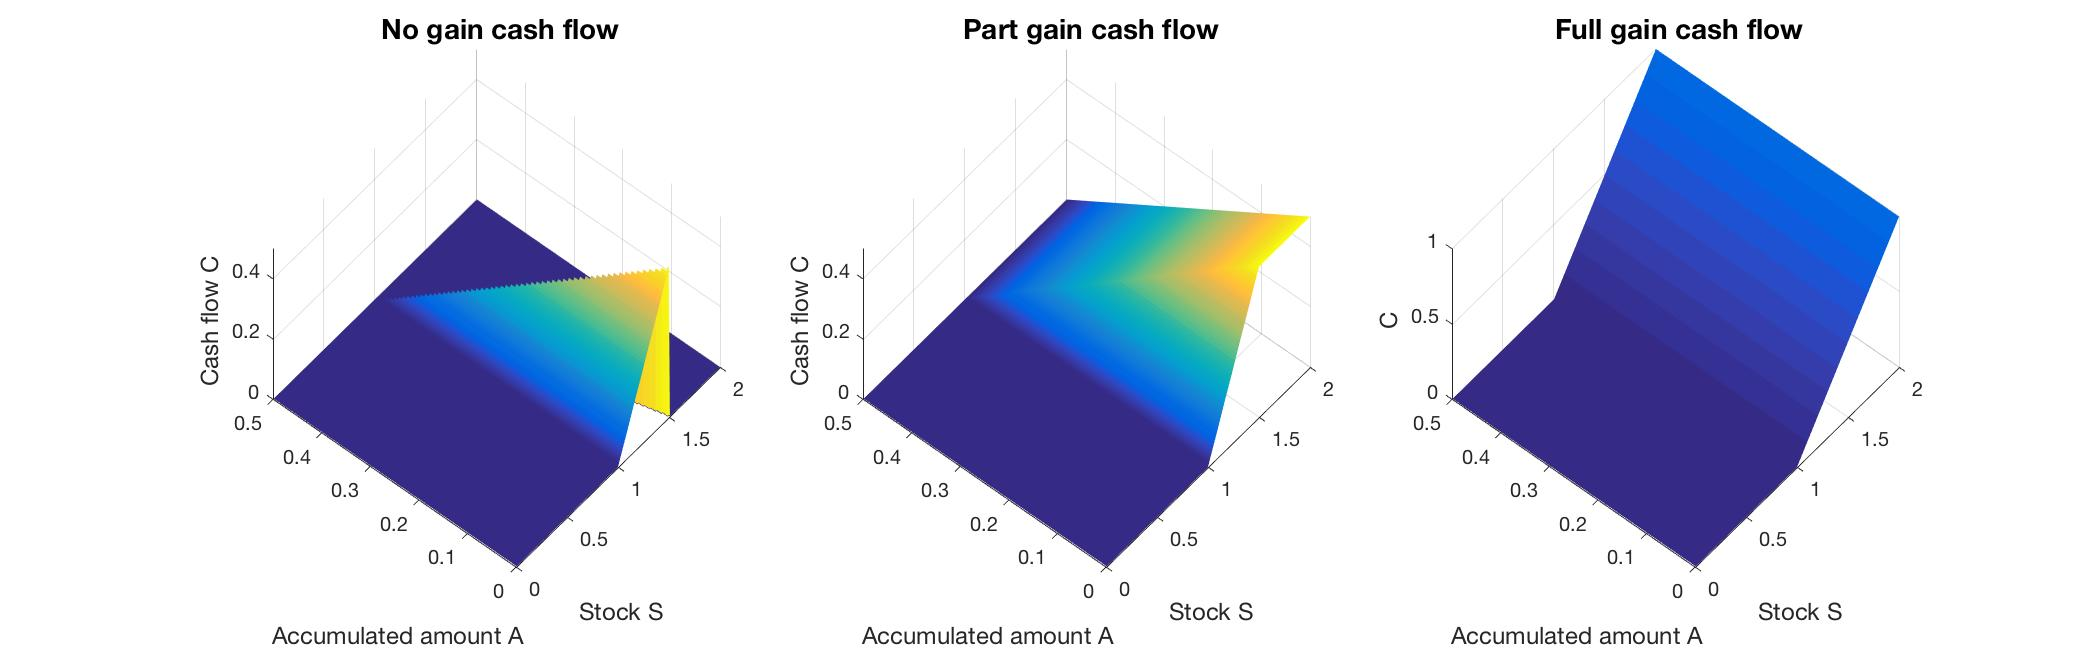
\includegraphics[width=\textwidth]{gfx/Cash-flow}
	\caption{Positive cash flow that produces jump on a fixing date for different type of knock-out.}
	\label{fig:cash-flow}
\end{figure}

Finally, the net present value of FX-TARN in domestic currency for FX rate realization $\mathbf{S} = (S(t_1),S(t_2),\ldots,S(t_N))$ is
\begin{equation}\label{eq:intro:pv}
P(\mathbf{S}) =N_f \times \sum_{n=1}^N\frac{\mathbf{C}^\text{tot}_n(S(t_n),A(t_{n-1}))}{B_d(t_0,t_n)}, \qquad A(t_0)=0,
\end{equation}
where $B_d(t_0,t_n)^{-1}$ is the domestic discounting factor from $t_n$ to $t_0$ and $\mathbf{C}^\text{tot}_n = C_n(S(t_n),A(t_{n-1}))+C^\ast_n(S(t_n),A(t_{n-1}))$ is the total cash flow at time $t_n$.

\section{Example of Term Sheet}
\label{sec:intro:term_sheet}
In this section, we will give an example of a particular TARN called \textit{"Leveraged Foreign Exchange Target Accrual Redemption Note with Full Settlement"}, i.e. Full Gain FX-TARN with gear factor. Thus this is a Full Gain FX-TARN with gear factor. The term sheet has the following form.

\begin{longtable}{|l|l|} 
\hline
\textbf{USD/CHF FX-TARN} & \textbf{Key Characteristics of the Transaction} \\
\hline 
\hline
Instrument Type & Leverage FX Target Accrual Redemption Note (TARN) \\
\hline
Trade Date & 23 May 2017\\
\hline
Buyer of CHF & The Bank \\
\hline
Buyer of USD & The Client \\
\hline
Underlying & USD/CHF Foreign Exchange rate\\
\hline
Notional Amount & USD 2'080'000.00 \\
&(versus maximum notional amount USD 4'160'000.00)\\
\hline
Accrual Amount & USD 40'000.00\\
per Fixing Date &(versus Leveraged Accrual Amount USD 80'000.00)\\
\hline
Leverage factor &2\\
\hline
Initial Spot Price & 0.9730 CHF per USD\\
\hline
Strike Price & As per date schedule below\\
\hline
Target Redemption Level & 0.4 CHF per 1 USD\\
\hline
Weekly Gains & On each Fixing Date, \\
& $\bullet$ If USD/CHF > Strike Price :\\
& \qquad Weekly Gains = USD/CHF - Strike Price\\ 
& $\bullet$ Otherwise :\\
& \qquad Weekly Gains = 0 CHF\\
\hline
Cumulated Gains & In respect of any Fixing Date, the Weekly Gains \\
& on that Fixing Date plus the sum of all Weekly \\
& Gains in respect of all previous Fixing Dates.\\
\hline
Redemption Event & A Redemption Event is deemed to have occurred \\
& if the Cumulated Gains (including the present fixing)\\ 
& is greater than or equal to the Target Redemption Level\\ 
& on any Fixing Date.\\
\hline
Expiration Date & 22 May 2018 \\
\hline
Fixing Reference & Weekly (Business Days)\\
\hline
Fixing Dates & 52 Fixings (see Schedule below)\\
\hline
Profile on Fixing Date & In respect of each Fixing Date :\\
& \textbf{1)} If no Redemption Event occurs and the Fixing Price is :\\
& $\quad\bullet$ At or above the Strike Price, the Client will buy from \\
& \qquad the Bank the Accrual Amount at the strike price : \\
& $\hspace{2cm}$ \textbf{Strike Price x Accrual Amount}\\
& Or \\
& $\quad\bullet$ Below the Strike Price, the Client will buy from the \\
& \qquad Bank the Leveraged Accrual Amount at the Strike  \\
& \qquad Price at the Strike Price for delivery on the relevant \\
& \qquad Settlement Date :\\
& $\hspace{1cm}$ \textbf{Leveraged Factor x Strike Price x Accrual Amount}\\
& \textbf{2)} If a Redemption Event occurs :\\
& $\quad\bullet$ The Client will buy from the Bank the Accrual Amount \\
& \qquad at the Strike Price for the Fixing Date that Redemption \\
& \qquad Event is deemed to have occurred : \\
& $\hspace{2cm}$ \textbf{Strike Price x Accrual Amount}\\
& $\quad\bullet$ The product is then knocked out for all remaining\\ 
& \qquad subsequent Fixings. There will be no further\\ 
&\qquad obligations between the Client and the Bank. \\
\hline
Schedule & \\
& \qquad\qquad$\begin{array}{|c|c|c|} 
\hline
\textbf{Fixing} & \textbf{Fixing Date} & \textbf{Strike Level} \\
\hline 
1 & 30 \text{ May } 2017 & 0.9275\\
2 & 6 \text{ June } 2017 & 0.9275\\
3 & 13 \text{ June } 2017 & 0.9350\\
4 & 20 \text{ June }2017 & 0.9350\\
5 & 27 \text{ June }2017 & 0.9350\\
6 & 4 \text{ July }2017 &  0.9420\\
7 & 18 \text{ July }2017 & 0.9420\\
8 & 25 \text{ July }2017 & 0.9420\\
\vdots & \vdots & \vdots\\
50 & 8 \text{ May }2018 & 0.9420\\
51 & 15 \text{ May }2018 & 0.9420\\
52 & 22 \text{ May }2018 & 0.9420\\
\hline
\end{array}$ \\
 & (Pay intention about the strike that is increasing in time.)\\
\hline
\caption{FX-TARN Term Sheet example.}
\end{longtable}



\section{Overview of the Thesis}
\label{sec:intro:overview}
This thesis is organized as follow. In the Chapter \ref{sec:Levy}, we introduce the L\'evy processes used to model the asset price. We also present the main mathematical properties that are useful in the pricing methods we will study.

In the Chapter \ref{sec:models}, we deal with the financial models such as jump-diffusion and pure jump models. We will see in particular the finite activity models of Merton and Kou. Then we will devote some time to the Normal Inverse Gaussian (NIG) and Variance Gamma (VG) models, that are special cases of infinite activity models. The tools characterizing the L\'evy processes such as the L\'evy densities and characteristic functions are respectively very useful in the Finite Difference method and the Convolution method.

In the Chapter \ref{sec:methods}, we expose the three numerical methods, which are the Monte Carlo method, the Finite Difference method and the Convolution method, used to price our exotic options. 

In the Chapter \ref{sec:calibration}, we calibrate all the models with respect to the market data in oder to be able to price the real term sheet of FX-TARN presented before.

The Chapter \ref{sec:results} is devoted to the results of experimental options. This allows us to analysis the performances of the tree different methods. Then, this chapter ends up with the pricing of our real case example.

Finally, the Chapter \ref{sec:conclusion} conclude this thesis with an overview of possible future works.
